% =====================================================================================
% Topic 34 (Lane B / B1) -- Journal of Network and Computer Applications (Elsevier)
% elsarticle, single column, review mode.  Build: pdflatex x2 + bibtex + pdflatex.
%
% TOOLCHAIN LAW (C6): every measured number comes from numbers.tex, which is generated by
% code/make_numbers.py from results/*.json.  Nothing numeric is typed by hand in this file.
% REFERENCE LAW (C5): refs.bib is generated by Submission_JNCA/make_bib.py from
% refs_verified.json; every entry carries a resolvable DOI printed on the page.
% =====================================================================================
\documentclass[preprint,review,12pt]{elsarticle}

\usepackage[T1]{fontenc}
\usepackage[utf8]{inputenc}
\usepackage{amsmath,amssymb,amsthm}
\usepackage{graphicx}
% Resolve figures whether main.tex sits next to figures/ (submission package, local build) or one
% level below it (code repository layout, where figures/ is at the repository root).
\graphicspath{{./}{../}}
\usepackage{booktabs}
\usepackage{multirow}
\usepackage{algorithm}
\usepackage{algpseudocode}
\usepackage{url}
\usepackage[hidelinks]{hyperref}

\journal{Journal of Network and Computer Applications}

% numbers.tex -- GENERATED by code/make_numbers.py on 2026-09-07. DO NOT EDIT BY HAND.
%% Every measured value in main.tex comes from results/*.json (law C6).
%% Regenerate:  python code/make_numbers.py

\newcommand{\numBuildDate}{2026-09-07}
\newcommand{\numCapCostPct}{12}
\newcommand{\numCapLatSixteen}{15}
\newcommand{\numCapLatSixtyfour}{63}
\newcommand{\numCapMissSixteen}{0.237}
\newcommand{\numCapMissSixtyfour}{0.212}
\newcommand{\numCfiveCells}{297}
\newcommand{\numCfiveDraftFail}{0}
\newcommand{\numCfiveFail}{0}
\newcommand{\numCfourRatioMax}{2.000}
\newcommand{\numCfourRatioMean}{1.272}
\newcommand{\numCfourTrials}{4,000}
\newcommand{\numConeMmax}{39}
\newcommand{\numConeN}{37}
\newcommand{\numConeRhoMin}{0.85897}
\newcommand{\numConservPct}{26.8}
\newcommand{\numConservRefused}{121}
\newcommand{\numConservSched}{451}
\newcommand{\numCsixGapMax}{1.82}
\newcommand{\numCsixGapMean}{0.17}
\newcommand{\numCsixGapPninefive}{1.08}
\newcommand{\numCsixOptFrac}{70.0}
\newcommand{\numCsixTrials}{200}
\newcommand{\numCthreeBandFeasible}{0}
\newcommand{\numCthreeBand}{12}
\newcommand{\numCthreeCells}{130}
\newcommand{\numCthreeQtwo}{82}
\newcommand{\numCtwoCells}{36}
\newcommand{\numCtwoClean}{29}
\newcommand{\numCtwoExact}{29}
\newcommand{\numEactiveMJ}{290.8}
\newcommand{\numEfiveDensBusy}{0.660}
\newcommand{\numEfiveDensFactor}{11}
\newcommand{\numEfiveDensRej}{38.4}
\newcommand{\numEfiveDensViol}{0.375}
\newcommand{\numEfiveEdfBusy}{0.778}
\newcommand{\numEfiveEdfRej}{31.2}
\newcommand{\numEfiveEdfViol}{4.000}
\newcommand{\numEfiveHarmBusy}{0.786}
\newcommand{\numEfiveHarmViol}{0.988}
\newcommand{\numEfiveLamHigh}{0.080}
\newcommand{\numEfiveLamLevels}{5}
\newcommand{\numEfivePolicyCells}{5}
\newcommand{\numEfiveResBusy}{0.644}
\newcommand{\numEfiveResExtraRejOneIn}{13}
\newcommand{\numEfiveResExtraRejPP}{7.6}
\newcommand{\numEfiveResRej}{38.9}
\newcommand{\numEfiveResViol}{0.000}
\newcommand{\numEfiveResZeroCells}{5}
\newcommand{\numEfourCameras}{121}
\newcommand{\numEfourConfigs}{8}
\newcommand{\numEfourCorThreeAtLB}{2}
\newcommand{\numEfourCorThreeRatioMax}{1.45}
\newcommand{\numEfourCorThreeRatioMin}{1.00}
\newcommand{\numEfourCorThreeViol}{0}
\newcommand{\numEfourFfdMissCert}{2}
\newcommand{\numEfourFfdViolCam}{1}
\newcommand{\numEfourFfdWorse}{4}
\newcommand{\numEfourHTwelveBoxes}{23}
\newcommand{\numEfourHTwelveLB}{21}
\newcommand{\numEfourUEightBoxes}{16}
\newcommand{\numEfourUEightFfd}{21}
\newcommand{\numEfourUEightLB}{16}
\newcommand{\numEidleMJ}{30.4}
\newcommand{\numEoneBelowN}{330}
\newcommand{\numEoneBelowUnsched}{0}
\newcommand{\numEoneEdfEightPct}{44}
\newcommand{\numEoneEdfSeventyPct}{21}
\newcommand{\numEoneEdfSeventy}{0.21}
\newcommand{\numEoneHarmEightPct}{91}
\newcommand{\numEoneHarmNinePct}{52}
\newcommand{\numEoneInstances}{594}
\newcommand{\numEoneUndecided}{6}
\newcommand{\numEoneWheelCands}{387}
\newcommand{\numEoneWheelEightPct}{97}
\newcommand{\numEoneWheelNinePct}{74}
\newcommand{\numEsixCells}{144}
\newcommand{\numEsixCorrect}{144}
\newcommand{\numEsixSeeds}{8}
\newcommand{\numEthreeCells}{28}
\newcommand{\numEthreeCorrect}{28}
\newcommand{\numEtwoBoundErr}{0.020}
\newcommand{\numEtwoCertMissed}{0}
\newcommand{\numEtwoCertTotal}{286,100}
\newcommand{\numEtwoEdfCertMissed}{1,568}
\newcommand{\numEtwoEdfCertTotal}{343,502}
\newcommand{\numEtwoEdfHetRuns}{384}
\newcommand{\numEtwoEdfHetViolRuns}{296}
\newcommand{\numEtwoEdfRuns}{576}
\newcommand{\numEtwoEdfUnifViolRuns}{0}
\newcommand{\numEtwoEdfViolRuns}{296}
\newcommand{\numEtwoFeasRunsInt}{192}
\newcommand{\numEtwoGainMaxPct}{43}
\newcommand{\numEtwoGainMinPct}{17}
\newcommand{\numEtwoHarmFeasInt}{129}
\newcommand{\numEtwoLatShapedMax}{63}
\newcommand{\numEtwoLatUnifMax}{23}
\newcommand{\numEtwoWheelCertMissed}{0}
\newcommand{\numEtwoWheelCertTotal}{302,224}
\newcommand{\numEtwoWheelFeasInt}{144}
\newcommand{\numEvBmc}{261}
\newcommand{\numEvCdnet}{2,516}
\newcommand{\numEvLasiesta}{936}
\newcommand{\numEvents}{3,713}
\newcommand{\numFrames}{166,589}
\newcommand{\numGainBmc}{44.4}
\newcommand{\numGainCdnet}{25.9}
\newcommand{\numGainLasiesta}{24.0}
\newcommand{\numGainMax}{3.08}
\newcommand{\numGainMin}{1.31}
\newcommand{\numHoldoutCells}{12}
\newcommand{\numHoldoutGain}{12.3}
\newcommand{\numHoldoutTotal}{121}
\newcommand{\numHoldoutVideos}{61}
\newcommand{\numHoldoutWins}{12}
\newcommand{\numMeanBmc}{111.7}
\newcommand{\numMeanCdnet}{32.9}
\newcommand{\numMeanLasiesta}{15.5}
\newcommand{\numMedBmc}{4}
\newcommand{\numMedCdnet}{2}
\newcommand{\numMedLasiesta}{10}
\newcommand{\numOracleGain}{19.4}
\newcommand{\numOracleShare}{36}
\newcommand{\numPerDsCells}{36}
\newcommand{\numPerDsWins}{36}
\newcommand{\numPninetyBmc}{160}
\newcommand{\numPninetyCdnet}{32}
\newcommand{\numPninetyLasiesta}{10}
\newcommand{\numRRMissSix}{0.299}
\newcommand{\numRROursSix}{0.455}
\newcommand{\numRefsOK}{30}
\newcommand{\numRefsPreprint}{4}
\newcommand{\numRefsTotal}{30}
\newcommand{\numShaAct}{8b87d704a51a}
\newcommand{\numShaEvents}{8fade8f15bbb}
\newcommand{\numTwelveHalfGain}{3.08}
\newcommand{\numTwelveHalfPrivate}{41.2}
\newcommand{\numTwelveHalfShared}{13.4}
\newcommand{\numVidBMC}{20}
\newcommand{\numVidCDnet}{53}
\newcommand{\numVidLASIESTA}{48}
\newcommand{\numVideos}{121}
   % generated by code/make_numbers.py -- do not edit by hand

% Repository coordinates live in their own generated file (repo.tex) so that publishing the code
% does not change the commit hash the paper quotes. The defaults below keep the document
% buildable for anyone who clones the repository, where repo.tex is absent.
\newcommand{\numRepoUrl}{\TODO{repository URL}}
\newcommand{\numRepoCommit}{\TODO{repository commit}}
\newcommand{\numRepoTag}{\TODO{repository tag}}
\IfFileExists{repo.tex}{\input{repo}}{}

% placeholder marker: the render check requires zero of these on the final PDF
\newcommand{\TODO}[1]{\textbf{[TODO: #1]}}

\newtheorem{theorem}{Theorem}
\newtheorem{lemma}[theorem]{Lemma}
\newtheorem{proposition}[theorem]{Proposition}
\newtheorem{corollary}[theorem]{Corollary}
\theoremstyle{definition}
\newtheorem{definition}[theorem]{Definition}
\newtheorem{remark}[theorem]{Remark}

\newcommand{\Nc}{N}
\newcommand{\Ki}{K_i}
\newcommand{\dens}{\rho}
\newcommand{\sched}{\sigma}
\newcommand{\Dur}{D}
\newcommand{\Lat}{L}
\newcommand{\pos}[1]{(#1)_{+}}

\begin{document}

\begin{frontmatter}

\title{How Many Cameras Can One Edge Box Certify?\\
Density-Based Admission Control, Budget Shaping and Fleet Dimensioning\\
for Shared-Accelerator Video Analytics}

\author[fsb]{Dat Lam Quoc\corref{cor1}}
\ead{lamquocdat@gmail.com}
\cortext[cor1]{Corresponding author. ORCID: 0009-0004-5432-9343.}
\address[fsb]{FPT School of Business and Technology, FPT University,
Ho Chi Minh City, Viet Nam}

\begin{abstract}
An edge box running object detection for a camera fleet has one accelerator and many streams, so
an operator must size it before installing anything: how many cameras can this box serve while
still guaranteeing that no sufficiently long event is missed? The question has a one-line answer.
If camera $i$ is inspected at least once in every window of $\Ki$ frame slots --- a
\emph{refresh certificate} bounding its worst-case detection latency by $\Ki-1$ --- then a
schedule meeting every certificate exists whenever the fleet density
$\dens=\sum_i 1/\Ki$ is at most $5/6$, and no better rule exists without solving an intractable
instance. This is a Liu--Layland-style design rule for edge video
analytics: one addition decides admission in $O(1)$ time. Our central finding is that the test
alone is not enough. Under camera churn it still leaves \numEfiveDensViol\ certificate violations
per 1000 slots; pairing it with a constructive divisor-wheel scheduler removes them entirely, at
the cost of refusing \numEfiveResRej\,\% of admission requests. We add a convex rule for
allocating the density budget across cameras with different event-duration laws, a dimensioning
rule for multi-box deployments, and capacity reductions for model-switch cost and for
vision--language-model escalation blackouts. On a public corpus of \numVideos\
surveillance videos with \numEvents\ annotated events, the constructive scheduler misses
\numEtwoCertMissed\ of \numEtwoCertTotal\ certified events, while lazy EDF breaks the certificate
in \numEtwoEdfHetViolRuns\ of \numEtwoEdfHetRuns\ runs with heterogeneous windows. Budget shaping
cuts missed short events by \numHoldoutGain\,\% out of sample at unchanged energy.
\end{abstract}

\begin{keyword}
edge video analytics \sep resource management \sep admission control \sep shared accelerator \sep
worst-case guarantees \sep camera fleets \sep energy efficiency
\end{keyword}

\end{frontmatter}

% =====================================================================================
\section{Introduction}\label{sec:intro}

An edge box deployed in a building, a factory or a road segment typically carries one inference
accelerator and receives frames from tens of cameras. It cannot run a detector on every frame of
every camera; it must choose, slot by slot, which camera to inspect. Every deployment therefore
begins with a sizing question that today is answered by trial and error: \emph{how many cameras
can this box carry?}

The question only has a crisp answer once one fixes what ``carry'' means. Average accuracy is not
enough: an operator who installs a camera to detect intrusions needs to know what the system
guarantees in the worst case, not on average. We adopt the guarantee used by the companion work
on single-camera frame skipping: camera $i$ is served with a \emph{refresh certificate} of window
$\Ki$ if the accelerator inspects one of its frames at least once in every window of $\Ki$
consecutive slots. A certificate of window $\Ki$ is exactly the statement that every event on
camera $i$ lasting at least $\Ki$ slots is detected, with detection latency at most $\Ki-1$
slots. It is a per-camera service-level agreement expressible in one integer.

With that definition the fleet-sizing question becomes a scheduling feasibility question, and it
turns out to have a Liu--Layland-style answer. Write $\dens=\sum_{i}1/\Ki$ for the fleet
\emph{density}: the fraction of accelerator slots the certificates demand. Then

\begin{center}
\fbox{\parbox{0.86\linewidth}{\centering
$\dens\le 5/6$ $\Rightarrow$ a schedule meeting \emph{every} certificate exists,\\
and $5/6$ cannot be improved without solving the instance.}}
\end{center}

\noindent
One addition decides admission. The operator never has to construct a schedule to know whether a
fleet is feasible, and a camera can be admitted or refused online in $O(1)$ time. The
sufficiency at $5/6$ is a recent result in scheduling theory \cite{kawamura2024stoc,kawamura2026pnas};
the tightness is elementary and we prove it in Section~\ref{sec:capacity}. Our contribution is not
that theorem but what an edge-video-analytics system can be built out of it, and what the
guarantee costs once real event statistics, real model-switching costs and real escalation traffic
are put back in.

\paragraph{Contributions}
\begin{enumerate}
\item \textbf{A certified capacity law and an $O(1)$ admission test for camera fleets}
      (Section~\ref{sec:capacity}), together with a constructive $O(\Nc K)$ scheduler that
      \emph{realises} the schedule rather than merely proving it exists. We show empirically that
      this distinction matters: the density test alone reduces certificate violations under churn
      by about $\numEfiveDensFactor\times$, but only the test \emph{combined with} the constructive
      scheduler drives them to zero (Section~\ref{sec:eval-churn}).
\item \textbf{Budget shaping} (Section~\ref{sec:shaping}): given the empirical event-duration law
      of each camera, allocating the density budget by a water-filling rule minimises the expected
      number of \emph{uncertified} (too-short) events that are missed. This is a convex program
      whose optimality condition says that a camera's marginal value is its weighted expected
      duration mass below its current window. Fitted on past data and replayed on unseen data it
      reduces misses by \numHoldoutGain\,\% at identical energy.
\item \textbf{A dimensioning rule for multi-box deployments} (Section~\ref{sec:dimensioning}):
      rounding each window down to a power of two and packing by first-fit-decreasing yields a
      certified partition of the fleet across edge boxes using at most $\lceil 2\dens\rceil$
      boxes, within a factor two of any feasible partition, with every box schedulable by the
      constructive scheduler. We present this as a usable rule of thumb rather than a tight
      result: on our fleet it lands within
      \numEfourCorThreeRatioMin--\numEfourCorThreeRatioMax\ times the lower bound, and it is
      \emph{not} the best packing we measured (Section~\ref{sec:eval-dimensioning}).
\item \textbf{Capacity under two edge realities} (Section~\ref{sec:extensions}): model-switch cost
      $s$ divides capacity exactly by $1+s$ for a homogeneous fleet, and grouping cameras by model
      recovers most of it; vision--language-model escalation blackouts subtract from the
      \emph{window}, not from the density, with a closed-form budget.
\end{enumerate}

\paragraph{Evaluation}
All results are replayed on a public corpus of \numVideos\ surveillance videos
(CDnet2014, LASIESTA, BMC) with \numEvents\ annotated events over \numFrames\ frames, and all
numbers in this paper are produced programmatically from the released JSON result files. Energy
is reported in absolute millijoules using two constants measured on a Jetson Orin Nano in the
companion work. We report the uncomfortable findings as prominently as the favourable ones: the
$5/6$ rule is a good \emph{admission} rule but a poor \emph{bin-packing} rule
(Section~\ref{sec:eval-dimensioning}); our constructive scheduler cannot realise every schedule
the $5/6$ theorem promises; and roughly \numOracleShare\,\% of the benefit of budget shaping
disappears once the windows must be fitted on past data instead of on the evaluation data
(Section~\ref{sec:eval-sensitivity}).

\paragraph{Relation to companion work}
This paper reuses, with declaration, two artefacts of a companion single-camera study that is
currently under review: the event corpus described above, and the two energy constants
$E_{\mathrm{idle}}=\numEidleMJ$\,mJ and $E_{\mathrm{active}}=\numEactiveMJ$\,mJ per slot
(Section~\ref{sec:eval-energy}). No figure, table or numerical result of that work is reproduced
here, and no new hardware measurement is claimed. Lemma~\ref{lem:transfer} imports its
single-camera certificate theorem as a premise and does not reprove it. The present paper is
about the \emph{fleet}: capacity, admission, allocation and dimensioning across cameras, none of
which appears in the companion work.

% =====================================================================================
\section{Related work}\label{sec:related}

\subsection{Edge video analytics and accelerator sharing}
Edge video analytics systems optimise configuration, placement and offloading to maximise average
accuracy or throughput under a latency budget; see \cite{zhou2023comst} for a survey. SplitStream
\cite{liang2024splitstream} distributes multi-camera analytics across heterogeneous edge nodes with
a workload-adaptive split, formulated as an NP-hard optimisation and solved heuristically. FlexDO
\cite{queiroz2024flexdo} offloads DAG applications to edge resources with a flexible scheduling
algorithm evaluated on production traces. Recent work on multi-tenant DNN inference for
autonomous-vehicle perception \cite{liu2026multitenant} shares one GPU among several perception
streams and reduces fusion delay and its variability. Real-time GPU scheduling for DNN workloads
\cite{yang2022rtgpu} provides response-time analysis for parallel tasks with hard deadlines.

All of these optimise an \emph{average} objective or analyse \emph{job deadlines}. None of them
answers ``how many cameras fit'' with a closed-form test, and none carries a per-camera
worst-case coverage guarantee of the form we use. The distinction between a job deadline and a
coverage window matters: a periodic task with a deadline guarantees that a job released at a known
time completes on time, whereas an event in a video stream starts at an unknown phase, so what is
needed is that \emph{every} window of $\Ki$ slots contains an inspection.

\subsection{Attention scheduling for perception}
The closest prior work in spirit is attention scheduling for embedded perception
\cite{liu2023attention}, which schedules a detector's attention over multiple regions of interest
\emph{within one camera stream} and minimises a generalised uncertainty measure. It is the only
perception paper we found that cites the coverage-scheduling literature at all, and it cites it
only in passing: it does not use a density threshold and gives no capacity theorem. The unit of
scheduling there is a region inside one image; ours is a camera inside a fleet.

\subsection{Coverage scheduling theory}
The feasibility question behind our capacity law is the pinwheel problem
\cite{holte1989pinwheel}: given windows $K_1,\dots,K_\Nc$, produce an infinite sequence over
$\{1,\dots,\Nc\}$ in which symbol $i$ appears at least once in every $\Ki$ consecutive positions.
Density at most $1$ is necessary; the sufficient thresholds improved from $1/2$
\cite{holte1989pinwheel} through $7/10$ \cite{chanchin1993schedulers,chanchin1992general} and
$3/4$ \cite{fishburn2002densities} to the conjectured and now proved $5/6$
\cite{kawamura2024stoc,kawamura2026pnas}. Instances with two distinct windows are schedulable
exactly when the density is at most $1$ \cite{holte1992two}, and with three distinct windows
$5/6$ is both sufficient and tight \cite{linlin1997three}. Deciding an arbitrary instance is not
possible in polynomial time under standard assumptions, although the problem is fixed-parameter
tractable in the number of tasks \cite{kobayashi2025isaac}. Recent variants extend the model to
real-valued periods \cite{fujiwara2026real}, to finitely many visits
\cite{kanellopoulos2025kvisits,kanellopoulos2026finite}, to covering rather than packing
\cite{kawamura2025covering}, and to tasks with durations \cite{kusano2026sofsem}; the related
bamboo garden trimming problem \cite{gasieniec2024bamboo} studies the same structure under a
growth objective. See also \cite{jacobs2014windows} for the windows-scheduling perspective.

This literature is, without exception, theoretical. Its stated applications are satellite ground
stations, machine maintenance, patrolling and packet scheduling. We are not aware of any prior
work that instantiates it for camera scheduling or edge inference, and Table~\ref{tab:related}
positions the present paper against the nearest systems work.

\begin{table}[t]
\centering\small
\caption{Position of this paper. ``Capacity law'' means a closed-form test that decides how many
streams fit without constructing a schedule.}
\label{tab:related}
\begin{tabular}{llccc}
\toprule
Work & Scheduling unit & Guarantee & Capacity law & $O(1)$ admission \\
\midrule
SplitStream \cite{liang2024splitstream} & camera $\to$ node & average accuracy & no & no \\
Multi-tenant DNN \cite{liu2026multitenant} & inference request & predictability & no & no \\
Attention sched.\ \cite{liu2023attention} & region in one frame & mean uncertainty & no & no \\
RT GPU sched.\ \cite{yang2022rtgpu} & periodic job & job deadline & utilisation & no \\
Admission for BLE mesh \cite{leonardi2025racble} & connection & non-overlap & no & yes \\
\textbf{This paper} & \textbf{camera in a fleet} & \textbf{refresh window} & \textbf{$\dens\le5/6$} & \textbf{yes} \\
\bottomrule
\end{tabular}
\end{table}

\subsection{Admission control and dimensioning in networked systems}
Runtime admission control with a feasibility test is standard practice in real-time networking;
a recent example admits new connections on a Bluetooth Low Energy mesh only when the resulting
transmissions provably do not overlap \cite{leonardi2025racble}. Coverage guarantees with proved
complexity bounds also appear in sensor-network deployment, for instance exact polynomial-time
methods for $k$-strong barrier coverage \cite{binh2024barrier}, and periodic-interval design to
attain a theoretical minimum discovery latency \cite{cheng2026cpbis}. Our contribution is of the
same shape --- a feasibility test plus a construction plus a trace-driven evaluation --- applied
to a resource, the shared inference accelerator, where it has not been available. Our
dimensioning result uses the classical tight bound for first-fit-decreasing bin packing
\cite{dosa2007ffd} only as a point of comparison; the bound we prove comes from a different route
(Section~\ref{sec:dimensioning}).

% =====================================================================================
\section{System model and the refresh certificate}\label{sec:model}

\subsection{Architecture}
We consider one edge box hosting one inference accelerator and $\Nc$ cameras
(Figure~\ref{fig:system} describes the data path). Cameras push frames to a per-camera ring buffer;
a scheduler decides, once per accelerator service time, which camera's most recent frame is passed
to the detector. Frames not selected are dropped without being decoded at full resolution, so the
uplink and the decoder see a load proportional to the density rather than to the number of
cameras --- a side benefit we quantify in Section~\ref{sec:eval-energy}. A detection may trigger
an \emph{escalation}: a heavier model, typically a vision--language model, occupies the
accelerator for several consecutive slots. Section~\ref{sec:blackout} treats escalations.

\begin{figure}[t]
\centering
\fbox{\parbox{0.92\linewidth}{\centering\small\vspace{2mm}
\texttt{cameras $1..N$} $\longrightarrow$ \texttt{per-camera ring buffers (latest frame)}
$\longrightarrow$ \textbf{scheduler} $\sched(t)$ $\longrightarrow$ \texttt{shared accelerator}\\[1mm]
\texttt{detector (1 slot)} \quad $\mid$ \quad \texttt{escalation / VLM ($\ell$ slots, $\ge P_e$ apart)}\\[1mm]
admission test: admit camera with window $K_{\mathrm{new}}$ iff
$\dens + 1/K_{\mathrm{new}} \le \dens^\star$
\vspace{2mm}}}
\caption{Data path of the edge box. The scheduler is the only component this paper changes; the
admission test is the only state it keeps ($\dens$, one floating-point number, plus a residue
wheel of $O(K_{\max})$ bits for the constructive variant of Section~\ref{sec:constructive}).}
\label{fig:system}
\end{figure}

\subsection{Slots, schedules and certificates}
Time is slotted, $t\in\mathbb{N}$; one slot is the accelerator's per-frame service time for the
detector. A \emph{schedule} is a map $\sched:\mathbb{N}\to\{1,\dots,\Nc\}\cup\{\bot\}$: at slot
$t$ the accelerator runs the detector on the current frame of camera $\sched(t)$, or idles.

\begin{definition}[refresh certificate]\label{def:refresh}
$\sched$ has the \emph{$\Ki$-refresh property} for camera $i$ if every window of $\Ki$ consecutive
slots contains some $t$ with $\sched(t)=i$. The \emph{certificate} $\mathcal{C}_i=(\Ki)$ is the
statement that every event on camera $i$ of duration $\Dur\ge\Ki$ slots is detected, with
detection latency $\Lat\le\Ki-1$.
\end{definition}

\begin{lemma}[certificate transfer]\label{lem:transfer}
$\sched$ delivers $\mathcal{C}_i$ for every $i$ if and only if it has the $\Ki$-refresh property
for every $i$. The bound $\Ki-1$ is tight, and events with $\Dur<\Ki$ are not certifiable: some
schedule with the property misses them.
\end{lemma}
\begin{proof}
Apply the single-camera certificate theorem of the companion work to the set
$O_i=\{t:\sched(t)=i\}$: the refresh property places a service slot inside every interval of
$\Ki$ consecutive slots, hence inside any event of duration at least $\Ki$; tightness and the
counterexample for $\Dur<\Ki$ carry over unchanged.
\end{proof}

Lemma~\ref{lem:transfer} is the bridge that makes the rest of the paper a scheduling problem: a
per-camera perception guarantee is exactly a per-camera coverage window, and the accelerator is a
single server.

\subsection{What happens to the events that are too short}\label{sec:lemma2}
Certificates cover long events. In real surveillance corpora most events are short: in our corpus
the median event lasts \numMedCdnet\ frames on CDnet2014, \numMedLasiesta\ on LASIESTA and
\numMedBmc\ on BMC. A guarantee that covers only long events would be of limited use if nothing
could be said about the rest. The following lemma says that the same window $\Ki$ also yields a
distribution-free bound for the short ones, and identifies the worst schedule.

\begin{lemma}[periodic service is the worst refreshing schedule]\label{lem:worst}
Let $\sched$ have the $\Ki$-refresh property for camera $i$ and let its service gaps be
$g_1,g_2,\dots\le\Ki$. Under a uniformly random event phase, an event of duration $\Dur$ is missed
with probability
\[
\Pr(\text{miss}\mid \Dur)\;=\;\frac{\sum_j \pos{g_j-\Dur}}{\sum_j g_j}\;\le\;\pos{1-\Dur/\Ki},
\]
so that $\Pr(\text{miss}_i)\le \varepsilon_i(\Ki):=\mathbb{E}_{\Dur\sim F_i}\!\big[\pos{1-\Dur/\Ki}\big]$
for the camera's empirical duration law $F_i$. For every $\Dur<\Ki$ the inequality is an equality
if and only if all gaps equal $\Ki$, that is, if and only if service is exactly periodic.
\end{lemma}

The proof is in \ref{app:proofs}. Two consequences drive the rest of the paper. First, the design
objective $\varepsilon_i(K)=\mathbb{E}[\pos{1-\Dur/K}]$ is computable from a camera's history and
requires no model of the detector; Section~\ref{sec:shaping} minimises it under the density
budget. Second, because the bound is attained by periodic service and our constructive scheduler
\emph{is} periodic, the bound is not merely an upper bound but a prediction: in
Section~\ref{sec:eval-frontier} it matches the measured miss rate to within \numEtwoBoundErr.

% =====================================================================================
\section{Certified capacity and admission control}\label{sec:capacity}

\begin{definition}[profile, density]\label{def:profile}
A \emph{certificate profile} is a vector $A=(K_1,\dots,K_\Nc)\in\mathbb{N}_{\ge1}^{\Nc}$. It is
\emph{feasible} if a schedule with all $\Ki$-refresh properties exists. Its \emph{density} is
$\dens(A)=\sum_{i=1}^{\Nc}1/\Ki$.
\end{definition}

Feasibility of a certificate profile is precisely the pinwheel scheduling problem
\cite{holte1989pinwheel}: the certificate windows are the periods and the accelerator is the
single server.

\begin{theorem}[certified capacity]\label{thm:capacity}
Let $A$ be a certificate profile.
\begin{enumerate}
\item[(i)] (necessity) If $A$ is feasible then $\dens(A)\le1$.
\item[(ii)] (sufficiency) If $\dens(A)\le 5/6$ then $A$ is feasible \cite{kawamura2024stoc,kawamura2026pnas}.
\item[(iii)] (tightness) For every $\varepsilon>0$ there is an infeasible profile with
      $\dens(A)\le 5/6+\varepsilon$.
\end{enumerate}
Hence the \emph{certified capacity} of one accelerator --- the largest density admissible without
inspecting the structure of the profile --- is exactly $5/6$.
\end{theorem}

Part~(i) is a counting argument; part~(iii) has a four-line self-contained proof; both are in
\ref{app:proofs}. Part~(ii) is the density-threshold theorem. Its proof proceeds by computer
search over a large but finite family of instances, which has an operational consequence we return
to in Section~\ref{sec:constructive}: it certifies existence without providing a simple online
scheduler.

\begin{corollary}[homogeneous fleet]\label{cor:homog}
If every camera has the same window $K$ then $N_{\max}(K)=K$: round robin serves each camera every
$K$ slots, and $N>K$ violates Theorem~\ref{thm:capacity}(i). The $5/6$ margin is the price of
heterogeneity.
\end{corollary}

\begin{corollary}[online admission control]\label{cor:admission}
Maintain the density $\dens$ of the admitted fleet. Admit a new camera requesting window
$K_{\mathrm{new}}$ if and only if $\dens+1/K_{\mathrm{new}}\le5/6$. Every admitted fleet is
certifiable; the test is $O(1)$, needs no re-solve, and is monotone, so a camera that leaves
frees exactly $1/\Ki$ of budget.
\end{corollary}

\begin{proposition}[structured profiles]\label{prop:structured}
(a) If the windows form a divisibility chain (\emph{harmonic}: $K_{(1)}\mid K_{(2)}\mid\cdots$)
then $A$ is feasible if and only if $\dens(A)\le1$ \cite{holte1989pinwheel}.
(b) With two distinct windows, feasible if and only if $\dens\le1$ \cite{holte1992two}; with three
distinct windows, $\dens\le5/6$ suffices and is tight \cite{linlin1997three}.
(c) Rounding each $\Ki$ \emph{down} to $\hat K_i=2^{\lfloor\log_2\Ki\rfloor}$ preserves every
certificate and yields a harmonic profile, which is feasible whenever
$\sum_i 2^{-\lfloor\log_2\Ki\rfloor}\le1$ --- in particular whenever $\dens(A)\le1/2$.
\end{proposition}

\paragraph{Design consequence.} A fleet designer who is free to choose windows should choose them
harmonic: the accelerator then reaches density $1$ with a trivial schedule and no $5/6$ margin is
paid. A designer who must accept application-given windows gets $5/6$, and nothing better is
available without solving the instance, which cannot be done in polynomial time under standard
assumptions \cite{kobayashi2025isaac}. This is the same role that the utilisation bound plays for
rate-monotonic scheduling \cite{liulayland1973}: a conservative, instantaneous, composable test
that a system designer can actually use.

\subsection{A constructive scheduler}\label{sec:constructive}
Theorem~\ref{thm:capacity}(ii) guarantees existence. An edge box needs a schedule. We use the
\emph{residue wheel}: round each window down to $\hat K_i=2^{\lfloor\log_2 K_i\rfloor}$, fix a
wheel of $M$ slots with $M$ a power of two at least $\max_i\hat K_i$, and give camera $i$ a
residue class $r_i$ modulo $\hat K_i$ that is still free. Camera $i$ is then served at exactly the
slots $t\equiv r_i \pmod{\hat K_i}$, so its gap is exactly $\hat K_i\le K_i$ and its certificate
holds by construction. Because the $\hat K_i$ are powers of two they form a divisibility chain, so
a free residue class exists whenever the rounded density is at most $1$
(Proposition~\ref{prop:structured}(a)), and Algorithm~\ref{alg:admit} finds one in $O(M)$ time.

\begin{algorithm}[t]
\caption{Admission and service on one edge box}
\label{alg:admit}
\begin{algorithmic}[1]
\State \textbf{state:} occupancy bitmap $\mathrm{occ}[0..M-1]$, initially all free
\Procedure{Admit}{$K_{\mathrm{new}}$}
  \State $\hat K \gets 2^{\lfloor\log_2 K_{\mathrm{new}}\rfloor}$
  \For{$r \gets 0$ \textbf{to} $\hat K-1$}
     \If{$\mathrm{occ}[x]$ is free for all $x \equiv r \pmod{\hat K}$}
        \State mark those $x$ busy; \Return $(\hat K, r)$ \Comment{admitted}
     \EndIf
  \EndFor
  \State \Return \textsc{reject} \Comment{no free residue class: the box is full}
\EndProcedure
\Procedure{Serve}{$t$}
  \State \Return the unique admitted camera $i$ with $t \equiv r_i \pmod{\hat K_i}$, or $\bot$
\EndProcedure
\Procedure{Release}{$i$} \State mark the residues of camera $i$ free \EndProcedure
\end{algorithmic}
\end{algorithm}

Two properties make Algorithm~\ref{alg:admit} usable online. Residues of admitted cameras are
never reassigned, so a join or a departure cannot stretch anybody else's gap; and a camera
admitted at slot $t_0$ is first served within $\hat K_i$ slots, so its certificate holds from
admission. The price is that rounding down to a power of two can waste up to a factor two of
capacity, and that repeated joins and departures fragment the wheel. We measure both in
Section~\ref{sec:eval-churn}.

\subsection{Recovering the capacity lost to rounding: the divisor wheel}\label{sec:wheel}
Rounding to powers of two is wasteful when a window is just below one: a camera asking for
$K_i=13$ is served every $8$ slots, spending $62\,\%$ more accelerator share than it asked for.
The fix keeps the residue-wheel idea and drops the power-of-two restriction. Fix a wheel length
$M$; round each window down to the largest \emph{divisor} of $M$ that does not exceed it,
$d_i=\max\{d: d\mid M,\ d\le K_i\}$; then assign residue classes as before, now with
backtracking, since divisors of $M$ need not be pairwise divisible. Camera $i$ is served exactly
every $d_i\le K_i$ slots, so the certificate again holds by construction, and \emph{a successful
packing is itself the certificate} --- no density theorem is invoked at all. We try $M$ over
\numEoneWheelCands\ candidate wheel lengths (every $a\cdot2^j$, which subsumes the power-of-two
scheme, plus every $13$-smooth number up to $2520$) in increasing order of rounded density, and
keep the first that packs. With $M=2520$, for instance, a window of $13$ is rounded to $12$
rather than to $8$.

This is a strict improvement and costs only $O(\Nc M)$ offline work: on the random profiles of
Section~\ref{sec:eval-schedulability} the divisor wheel constructs a schedule for
\numEoneWheelEightPct\,\% of the band $\dens\in(0.75,5/6]$ against \numEoneHarmEightPct\,\% for
single-base rounding, and \numEoneWheelNinePct\,\% against \numEoneHarmNinePct\,\% just above the
threshold. The instances it still fails are those admitting no perfectly periodic schedule at
all, which no residue-wheel method can reach.

\begin{remark}[the constructive gap]\label{rem:gap}
A genuine gap remains between what Theorem~\ref{thm:capacity}(ii) promises and what a scheduler we
can implement delivers. The published constructive thresholds are $7/10$
\cite{chanchin1993schedulers} and $3/4$ \cite{fishburn2002densities}, and the $5/6$ proof is a
computer search over a finite family that yields no comparable online rule. We did not implement
the $7/10$ or $3/4$ schedulers; the divisor wheel above is our own construction, and we make no
claim that it dominates them. We report the resulting gap quantitatively rather than hiding it:
Section~\ref{sec:eval-schedulability} measures how often our scheduler fails on profiles that are
provably feasible, and Section~\ref{sec:eval-dimensioning} shows the gap costing real edge boxes.
\end{remark}

% =====================================================================================
\section{Allocating the density budget}\label{sec:shaping}

Corollary~\ref{cor:admission} says which fleets fit. It does not say what windows to give them.
If the operator --- rather than the application --- may choose $\Ki$, then the budget $5/6$ (or
$1$ for a harmonic profile) is a resource to be allocated, and Lemma~\ref{lem:worst} gives the
objective: minimise the expected number of uncertified events missed.

Let camera $i$ carry weight $w_i>0$ (its event rate, say) and empirical duration law $F_i$, and
write $x_i=1/\Ki$ for its slot share.

\begin{theorem}[certified budget shaping]\label{thm:shaping}
The relaxed allocation problem
\[
\min_{x\in(0,1]^\Nc}\ \sum_i w_i\,h_i(x_i)
\quad\text{s.t.}\quad \sum_i x_i\le\dens^{\star},
\qquad h_i(x):=\mathbb{E}_{\Dur\sim F_i}\!\big[\pos{1-x\Dur}\big],
\]
is a separable convex program. The budget constraint is tight at any optimum, and $x^\star$ is
optimal if and only if there is a multiplier $\lambda\ge0$ with
$\lambda\in w_i\,\partial(-h_i)(x_i^\star)$ for every $i$ with $x_i^\star<1$. Where $F_i$ has no
atom at $1/x_i^\star$ this is the water-filling condition
\[
w_i\,\mathbb{E}_{F_i}\!\big[\Dur\,\mathbf 1\{\Dur<1/x_i^\star\}\big]=\lambda .
\]
Setting $\dens^{\star}=5/6$ and $\Ki=\lceil 1/x_i^\star\rceil$ yields a certifiable profile by
Theorem~\ref{thm:capacity}(ii); setting $\dens^{\star}=1$ and rounding each $\Ki$ down to a power
of two yields a profile certifiable \emph{and} constructible by Algorithm~\ref{alg:admit}.
\end{theorem}

The proof is in \ref{app:proofs}. The subgradient form matters in practice because event durations
are integers, so each $h_i$ is piecewise linear and non-differentiable exactly at the interesting
points $x=1/d$.

\paragraph{Reading.} The marginal value of accelerator share to camera $i$ is its weighted expected
duration mass \emph{below its current window}. Cameras whose events are short and frequent receive
short windows; cameras whose events are long are served rarely at no certified cost, because their
events are certified anyway. In the companion single-camera work a per-scene window was ``real but
uncapturable'' online; here the allocation is a fleet-level, offline decision on calibrated
histories, so the headroom is actually spendable.

\paragraph{What we actually run.} We do not solve the continuous program. Because each $h_i$ is
convex, the gain per unit of density from shortening a camera's window is decreasing, so we use
\emph{greedy marginal allocation} on a discrete window grid: repeatedly buy the step with the best
ratio of objective reduction to density cost until the budget is exhausted. This is optimal for the
continuous relaxation but not for the grid, which is a knapsack. We measured the loss against
exhaustive enumeration on \numCsixTrials\ small instances with heavy-tailed duration laws: greedy
is exactly optimal on \numCsixOptFrac\,\% of them, and its objective is worse by
\numCsixGapMean\,\% on average, \numCsixGapPninefive\,\% at the 95th percentile and
\numCsixGapMax\,\% at worst. We therefore call the procedure greedy marginal allocation, not ``the
KKT solution''.

\paragraph{Capping certified latency.} Shaping gives long-event cameras large windows, which
raises their certified latency bound $\Ki-1$. An operator who needs a latency ceiling can simply
cap the grid at $K_{\max}$; Section~\ref{sec:eval-sensitivity} quantifies the cost, which is small.

% =====================================================================================
\section{Fleet dimensioning across edge boxes}\label{sec:dimensioning}

A fleet larger than one box can carry must be partitioned. The natural approach --- pack the
loads $1/\Ki$ into bins of capacity $5/6$ by first-fit-decreasing --- yields a certified partition
but no useful bound relative to the fleet's density, because the optimum of that bin-packing
problem can itself be twice $\lceil\dens\rceil$ (take every $\Ki=2$: the $5/6$ rule puts one
camera per box, while two cameras with $K=2$ share a box perfectly). We therefore take a different
route and obtain a bound.

\begin{corollary}[fleet dimensioning by harmonic rounding]\label{cor:dimensioning}
Let $A=(K_1,\dots,K_M)$ be the fleet profile, $\hat K_i=2^{\lfloor\log_2 K_i\rfloor}$ and
$x_i=1/\hat K_i$. Pack $\{x_i\}$ by first-fit-decreasing into bins of capacity $1$. Then
\begin{enumerate}
\item every bin is schedulable by Algorithm~\ref{alg:admit}, and every original certificate holds,
      because $\hat K_i\le K_i$;
\item the packing is perfect: the number of boxes is $m=\big\lceil\sum_i 1/\hat K_i\big\rceil$;
\item $m\le\lceil 2\dens(A)\rceil\le 2\lceil\dens(A)\rceil$;
\item any partition into feasible boxes needs $m^\star\ge\lceil\dens(A)\rceil$ boxes.
\end{enumerate}
Hence the procedure is within a factor two of optimal, and exactly optimal when the profile is
already harmonic.
\end{corollary}

The proof is in \ref{app:proofs}; item~2 uses the fact that dyadic item sizes are pairwise
divisible, for which first-fit-decreasing fills each bin exactly before opening the next. We
verified all four items on \numCfourTrials\ random profiles: the packing was perfect and every box
schedulable in all of them, and the realised ratio $m/\lceil\dens\rceil$ was
\numCfourRatioMean\ on average and \numCfourRatioMax\ at worst.

\begin{remark}
The factor two comes from the rounding, not from the $5/6$ threshold: it is the price of insisting
on a schedule we can construct. A hypothetical constructive $5/6$ scheduler would give
$\lceil 1.2\,\dens\rceil$. This is the fleet-level face of Remark~\ref{rem:gap}.
\end{remark}

% =====================================================================================
\section{Two edge realities: switch cost and escalation blackouts}\label{sec:extensions}

\subsection{Model-switch cost}\label{sec:switch}
Cameras may run different detectors. Switching the accelerator between two cameras with different
models costs $s$ slots of weight loading during which no frame is served.

\begin{proposition}[capacity under switch cost]\label{prop:switch}
Let $K_i'=\lfloor \Ki/(1+s)\rfloor$. If $\sum_i 1/K_i'\le 5/6$ then a schedule exists that delivers
every certificate under switch cost $s$. For a homogeneous fleet of $\Nc\ge2$ cameras with
pairwise distinct models, the capacity is exactly
\[
N_{\max}(K,s)=\big\lfloor K/(1+s)\big\rfloor .
\]
\end{proposition}

The sufficiency is a macro-slot construction and the converse is an amortised counting argument
over service runs; both are in \ref{app:proofs}. We checked the exact capacity by exhaustive state
search: on all \numCtwoClean\ configurations that the search decided, the measured capacity equals
$\lfloor K/(1+s)\rfloor$ exactly.

Switch cost is expensive: it divides capacity rather than reducing it. At $K=12$, a box serves
$12$ cameras with $s=0$, $6$ with $s=1$ and $4$ with $s=2$. The obvious mitigation is to let
cameras share models.

Partitioning the fleet into $q$ \emph{model groups}, so that switching inside a group is free,
recovers most of the loss: for a homogeneous window $K$ and $q\ge2$ groups, $\Nc+q\,s\le K$ is
sufficient and $\Nc+(q-1)\,s\le K$ is necessary, a sandwich of width exactly $s$ slots. The two
statements, their proofs and the exhaustive check that found no feasible configuration between
them are in \ref{app:groups}. The design consequence is worth stating plainly: at $K=24$ and
$s=3$, giving every camera its own model allows $6$ cameras per box; two model groups allow $18$;
one shared model allows $24$. Consolidating models buys more capacity than any scheduling
improvement available here.

\subsection{Escalation blackouts}\label{sec:blackout}
When a detection triggers a vision--language model, the accelerator is unavailable for $\ell$
consecutive slots. Assume escalations start at least $P_e$ slots apart, with $P_e\ge\ell$ so they
do not overlap; this is the rate limit an operator configures anyway.

\begin{proposition}[capacity under blackouts]\label{prop:blackout}
Let $B_i=\min\!\big(\Ki,\ \ell\lceil(\Ki+\ell-1)/P_e\rceil\big)$ and $K_i''=\Ki-B_i>0$. If
$\sum_i 1/K_i''\le5/6$ then a schedule exists delivering every certificate despite the escalations,
and it can be run online without any forecast of when escalations occur.
\end{proposition}

The proof (\ref{app:proofs}) counts the escalations that \emph{intersect} a window rather than
those that start in it --- an escalation beginning just before a window still consumes up to
$\ell-1$ of its slots --- and then runs the schedule on the subsequence of available slots,
advancing the pointer only when a slot is actually free. We checked the budget against the true
worst case over all escalation phases on \numCfiveCells\ combinations of $(\ell,P_e,K)$: it was
never optimistic (\numCfiveFail\ failures).

The operational reading is that escalations subtract from the \emph{window}, not from the density.
A vision--language call of $\ell=8$ slots once every $P_e=50$ slots removes $8$ slots from
\emph{every} window, so a box with $K=12$ can no longer certify $6$ cameras while one with $K=14$
still can.

\begin{remark}[real periods]\label{rem:realperiods}
If camera $i$ captures with frame period $\tau_i$ while the accelerator slot is $\tau_a$, a
certificate of $K^{(f)}_i$ camera frames is a window of $\Ki=\lfloor K^{(f)}_i\tau_i/\tau_a\rfloor$
slots. Flooring preserves the certificate and inflates the density by at most
$\sum_i\big(1/\Ki-\tau_a/(K^{(f)}_i\tau_i)\big)$. Without flooring the instance has real-valued
periods, for which the $5/6$ threshold is proved for up to three distinct values and conjectured in
general \cite{fujiwara2026real}. We use the floored form throughout and leave real periods to
future work.
\end{remark}

% =====================================================================================
\section{Evaluation}\label{sec:eval}

\subsection{Setup}\label{sec:eval-setup}
We replay a public corpus of \numVideos\ surveillance videos --- \numVidCDnet\ from CDnet2014
\cite{cdnet2014}, \numVidLASIESTA\ from LASIESTA \cite{lasiesta2016} and \numVidBMC\ from BMC
\cite{bmc2012} --- carrying \numEvents\ annotated events
over \numFrames\ frames, as $\Nc$ synchronous camera streams on one simulated accelerator. Onsets
and durations come from the event extraction of the companion work; the input files are pinned by
SHA-256 (\texttt{\numShaEvents\ldots}, \texttt{\numShaAct\ldots}). The three datasets have very
different duration laws (median / 90th percentile / mean, in frames: CDnet2014
\numMedCdnet/\numPninetyCdnet/\numMeanCdnet, LASIESTA
\numMedLasiesta/\numPninetyLasiesta/\numMeanLasiesta, BMC \numMedBmc/\numPninetyBmc/\numMeanBmc),
which we exploit in Section~\ref{sec:eval-sensitivity}. Every experiment uses seed 42, and every
number below is generated programmatically from the released JSON files.

\subsection{Is the density rule the right admission rule?}\label{sec:eval-schedulability}
We drew \numEoneInstances\ random profiles ($\Nc\in[3,8]$, $\Ki\in[2,14]$), decided each one
exactly by cycle search in the state graph, and compared three policies
(Figure~\ref{fig:e1}, left).

\begin{figure}[t]
\centering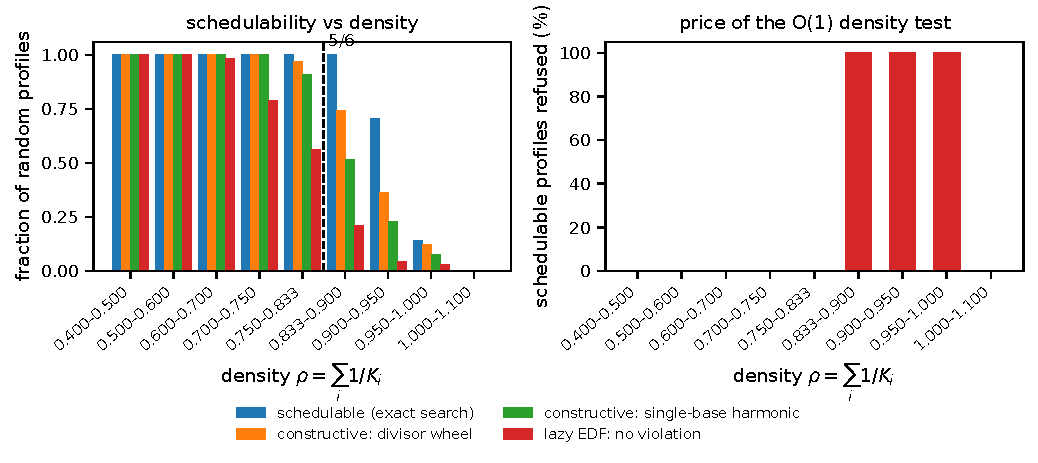
\includegraphics[width=\linewidth]{figures/fig_E1_schedulability.pdf}
\caption{Left: fraction of random profiles that are feasible, that our constructive scheduler
handles, and that lazy EDF runs without violating a window. Right: the price of the $O(1)$ test
--- the fraction of \emph{feasible} profiles it refuses, per density bin.}
\label{fig:e1}
\end{figure}

Three findings. First, the rule is sound in practice as well as in theory:
\numEoneBelowUnsched\ of the \numEoneBelowN\ profiles with $\dens\le5/6$ were infeasible.
Second, lazy earliest-deadline-first --- the heuristic an engineer would reach for --- is
\emph{not} a safe design rule: it violated a window on \numEoneEdfSeventyPct\,\% of profiles in
the band $(0.70,0.75]$ and \numEoneEdfEightPct\,\% in $(0.75,5/6]$, all of which are provably
feasible. Third, our constructive scheduler handles \numEoneHarmEightPct\,\% of the band
$(0.75,5/6]$, which is Remark~\ref{rem:gap} in numbers.

The right panel prices the conservatism. Below $5/6$ the test never refuses a feasible profile and
never admits an infeasible one; the entire cost sits above the threshold, where it refuses
\numConservRefused\ of \numConservSched\ feasible profiles overall, or \numConservPct\,\%. That
figure is a property of our sampling design, which deliberately over-weights the band above $5/6$,
and is not the refusal rate an operator would see on a natural fleet distribution; it is an upper
bound on the price of instantaneous admission.

\subsection{The energy--miss frontier and budget shaping}\label{sec:eval-frontier}
Figure~\ref{fig:e2} replays the corpus at four density budgets. Two results
(Table~\ref{tab:e2}). The constructive scheduler missed \numEtwoCertMissed\ of
\numEtwoCertTotal\ certified events across the whole experiment, and the certified latency bound
$\Ki-1$ held everywhere; lazy EDF, on the same profiles, missed \numEtwoEdfCertMissed\ of
\numEtwoEdfCertTotal\ certified events and broke a window in \numEtwoEdfHetViolRuns\ of the
\numEtwoEdfHetRuns\ runs with heterogeneous windows. (On a homogeneous profile lazy EDF
degenerates to round robin and never violates --- \numEtwoEdfUnifViolRuns\ violating runs ---
so the heterogeneous denominator is the informative one.) And
budget shaping reduces the uncertified miss rate by
\numEtwoGainMinPct--\numEtwoGainMaxPct\,\% at identical busy fraction, that is, at identical
energy. \textbf{That range is an in-sample upper bound}: here the windows were fitted on the same
events used to evaluate them. The figure to carry away is the out-of-sample one,
\numHoldoutGain\,\%, established in Section~\ref{sec:eval-sensitivity}; we quote the in-sample
range only to show how much of it is oracle.

Every comparison in this subsection is made at equal busy fraction, so ``fewer misses'' always
means ``fewer misses for the same energy''. Where a scheduler is work-conserving and therefore
spends the full energy budget regardless of $\dens^\star$, we say so explicitly
(Section~\ref{sec:eval-sensitivity}).

The bound of Lemma~\ref{lem:worst} predicted the measured miss rate to within \numEtwoBoundErr\
throughout, confirming that $\varepsilon_i(K)$ is usable as a design objective and not merely as a
loose bound.

The divisor wheel of Section~\ref{sec:wheel} was run on the same profiles: it missed
\numEtwoWheelCertMissed\ of \numEtwoWheelCertTotal\ certified events, and it constructed a
schedule for \numEtwoWheelFeasInt\ of the \numEtwoFeasRunsInt\ runs whose windows were shaped on
the integer grid, against \numEtwoHarmFeasInt\ for single-base rounding. The integer grid gives a
better objective than the harmonic grid but is harder to build; the divisor wheel closes part of
that gap.

\begin{figure}[t]
\centering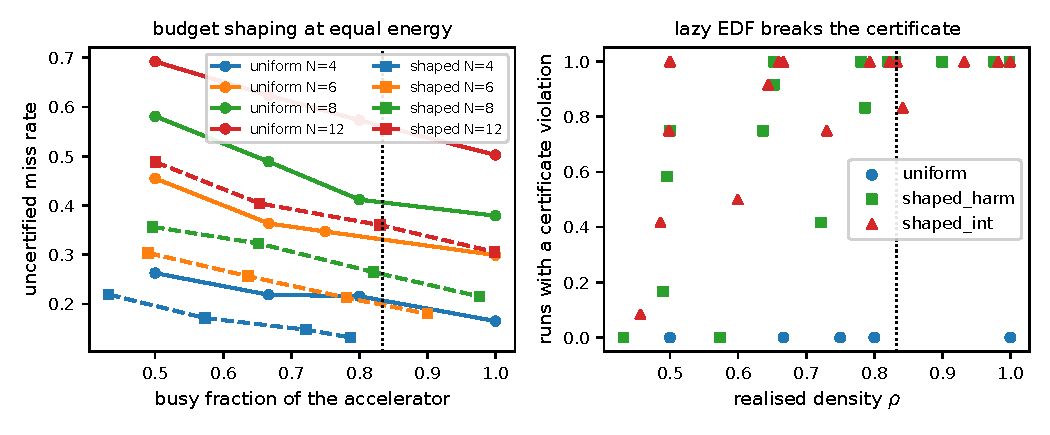
\includegraphics[width=\linewidth]{figures/fig_E2_frontier.pdf}
\caption{Left: uncertified miss rate against the accelerator's busy fraction, uniform versus
shaped windows at four density budgets. Right: fraction of runs in which lazy EDF violates a
certificate, against realised density.}
\label{fig:e2}
\end{figure}

\begin{table}[t]
\centering\small
\caption{Cost of the certificate, per configuration, at \emph{equal busy fraction} --- both
columns spend the same energy. Shaping trades certified latency for uncertified misses;
Section~\ref{sec:eval-sensitivity} caps the trade and gives the out-of-sample gain.}
\label{tab:e2}
\begin{tabular}{lcc}
\toprule
 & uniform windows & shaped windows \\
\midrule
busy fraction (energy) & $\dens^\star$ & $\dens^\star$ (equal by construction) \\
uncertified miss rate, in sample & baseline & $-\numEtwoGainMinPct$ to $-\numEtwoGainMaxPct$\,\% \\
uncertified miss rate, out of sample & baseline & $-\numHoldoutGain$\,\% \\
certified events missed & \numEtwoCertMissed & \numEtwoCertMissed \\
worst certified latency (slots) & \numEtwoLatUnifMax & \numEtwoLatShapedMax \\
\bottomrule
\end{tabular}
\end{table}

\subsection{The two edge realities: switch cost and blackouts}\label{sec:eval-switch}
Figure~\ref{fig:e36}(a) sweeps the switch cost for a homogeneous fleet of six cameras.
Proposition~\ref{prop:switch} predicted the outcome correctly in \numEthreeCorrect\ of
\numEthreeCells\ cells: where the condition holds, no run violated a certificate; where it fails,
every run did.

Figure~\ref{fig:e36}(b) sweeps escalation length $\ell\in\{2,4,8\}$ and rate limit
$P_e\in\{50,100,200\}$ for six cameras. Proposition~\ref{prop:blackout} predicted the outcome
correctly in \numEsixCorrect\ of \numEsixCells\ cells --- feasible configurations had no violation
in any run, infeasible ones violated in every run --- under exactly periodic escalations (the
tightest case, plotted) and equally under jittered ones (gaps drawn uniformly in $[P_e,2P_e)$,
omitted from the plot because the two panels coincide).

\begin{figure}[t]
\centering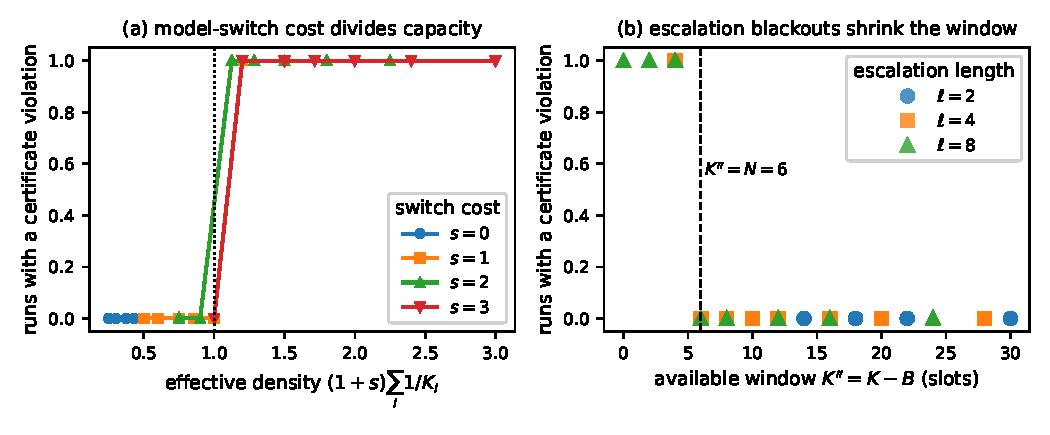
\includegraphics[width=\linewidth]{figures/fig_E36_extensions.pdf}
\caption{The two capacity reductions an edge deployment actually meets. (a) Certificate violations
against effective density $(1+s)\dens$ for model-switch costs $s\in\{0,1,2,3\}$. (b) Certificate
violations against the available window $K''=K-B$ under escalation blackouts, for escalation
lengths $\ell\in\{2,4,8\}$; the vertical line is $K''=\Nc$. Homogeneous fleet of six cameras in
both panels.}
\label{fig:e36}
\end{figure}

\subsection{How many edge boxes does a real fleet need?}\label{sec:eval-dimensioning}
We now treat all \numEfourCameras\ videos as \numEfourCameras\ cameras and ask how many edge boxes
they need, under a uniform profile and under a heterogeneous profile in which each camera's window
scales with its own median event duration. We compare Corollary~\ref{cor:dimensioning},
first-fit-decreasing into $5/6$-capacity boxes, and an EDF-fit heuristic that opens a new box when
lazy EDF starts violating (Figure~\ref{fig:e4}).

\begin{figure}[t]
\centering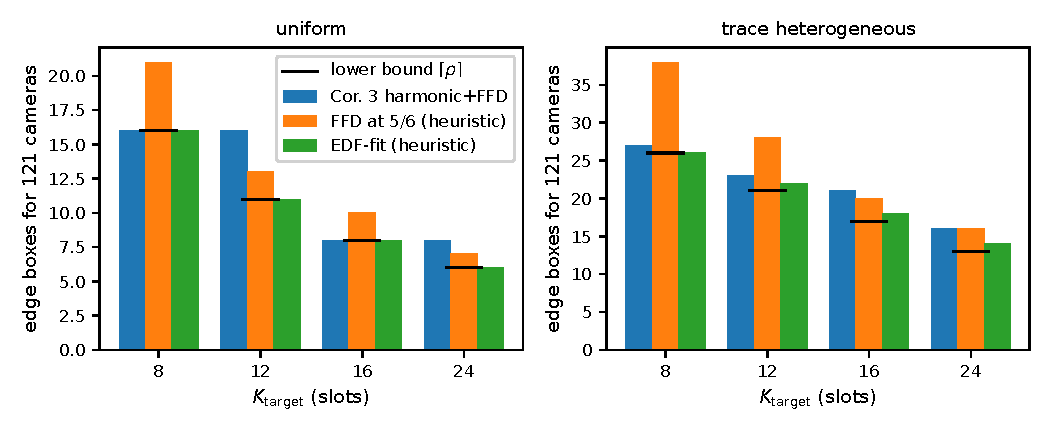
\includegraphics[width=\linewidth]{figures/fig_E4_dimensioning.pdf}
\caption{Edge boxes needed for \numEfourCameras\ cameras, against the target window. The black
marker is the information-theoretic lower bound $\lceil\dens\rceil$.}
\label{fig:e4}
\end{figure}

Corollary~\ref{cor:dimensioning} used between \numEfourCorThreeRatioMin\ and
\numEfourCorThreeRatioMax\ times the lower bound --- far inside its guarantee of two --- and hit
the lower bound exactly in \numEfourCorThreeAtLB\ of \numEfourConfigs\ configurations, with
\numEfourCorThreeViol\ certificate violations. Two findings run against intuition and we report
them as prominently as the favourable one.

\emph{The $5/6$ rule is a good admission rule but a poor packing rule.} Packing into
$5/6$-capacity boxes needed \emph{more} boxes than harmonic rounding in \numEfourFfdWorse\ of
\numEfourConfigs\ configurations, because a box of capacity $5/6$ simply holds less than a
harmonic box of capacity $1$. The threshold answers ``does this set fit'', not ``how should I
split this fleet''.

\emph{The constructive gap costs real certificates.} In one configuration a $5/6$ box satisfied
Theorem~\ref{thm:capacity}(ii) --- a schedule provably exists --- but our constructive scheduler
could not find it, forcing a fallback to EDF, which then missed \numEfourFfdMissCert\ certified
events on \numEfourFfdViolCam\ camera. This is not an implementation defect; it is
Remark~\ref{rem:gap} materialising as a service-level violation.

Finally, EDF-fit produced the smallest box counts, but its zero violations are not a guarantee:
the heuristic was fitted on the very trace and horizon used to evaluate it. Corollary
\ref{cor:dimensioning} needs no trace at all.

\subsection{Admission control under churn}\label{sec:eval-churn}
Cameras are installed and removed. We simulate a single box under Bernoulli join and departure
processes at \numEfiveLamLevels\ churn levels, comparing four policies: admit-then-EDF (admit
while $\dens\le1$ and rely on the scheduler), the $5/6$ density test, the harmonic density test at
threshold $1$, and Algorithm~\ref{alg:admit}, which combines a test with a construction
(Figure~\ref{fig:e5}, Table~\ref{tab:e5}).

\begin{figure}[t]
\centering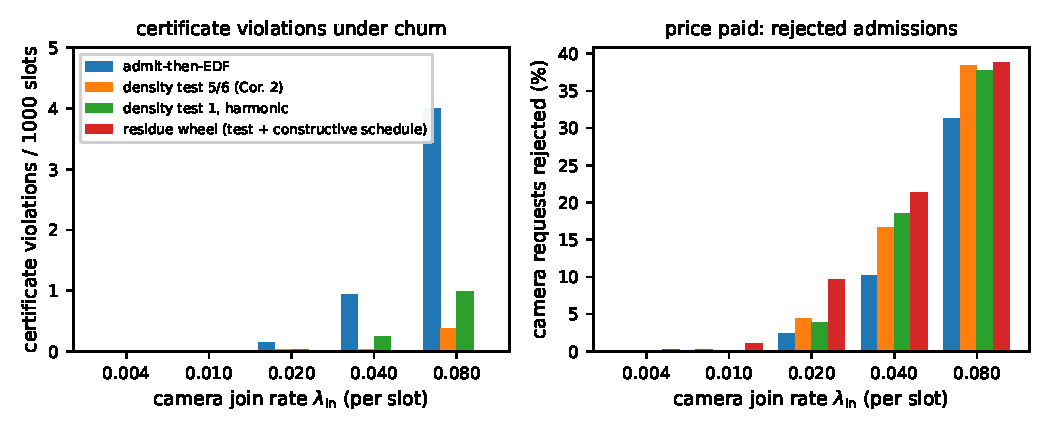
\includegraphics[width=\linewidth]{figures/fig_E5_churn.pdf}
\caption{Left: certificate violations per 1000 slots under camera churn. Right: the price paid ---
admission requests refused.}
\label{fig:e5}
\end{figure}

\begin{table}[t]
\centering\small
\caption{Admission policies at the highest churn level ($\lambda_{\mathrm{in}}=\numEfiveLamHigh$
joins per slot). A violation episode is a camera whose window elapsed without service. All four
policies are non-work-conserving, so the busy fraction column is a fair energy comparison.}
\label{tab:e5}
\begin{tabular}{lccc}
\toprule
policy & violations / 1000 slots & refused (\%) & busy fraction \\
\midrule
admit-then-EDF & \numEfiveEdfViol & \numEfiveEdfRej & \numEfiveEdfBusy \\
harmonic density test ($\dens\le1$) & \numEfiveHarmViol & --- & \numEfiveHarmBusy \\
density test ($\dens\le5/6$, Cor.~\ref{cor:admission}) & \numEfiveDensViol & \numEfiveDensRej & \numEfiveDensBusy \\
\textbf{Algorithm~\ref{alg:admit} (test + construction)} & \textbf{\numEfiveResViol} & \numEfiveResRej & \numEfiveResBusy \\
\bottomrule
\end{tabular}
\end{table}

This is the paper's central operational result, and it has three parts. Admit-then-EDF fails as
predicted, at \numEfiveEdfViol\ violations per 1000 slots. The admission test alone cuts that by
roughly \numEfiveDensFactor$\times$ --- but \emph{does not eliminate it}, because a sound test
guarantees that a schedule exists while an online EDF does not realise it. Only the test combined
with the constructive residue wheel reaches zero violations, and it does so at every one of the
\numEfiveResZeroCells\ churn levels.

The price is honest and visible in the right panel: Algorithm~\ref{alg:admit} refuses
\numEfiveResRej\,\% of requests at the highest churn level against \numEfiveEdfRej\,\% for
admit-then-EDF. Part of that gap is the power-of-two rounding and part is fragmentation of the
residue wheel after departures, which is a buddy-allocation effect. An operator buys a hard
guarantee with roughly one refused camera in thirteen.

\subsection{Energy in millijoules and the consolidation gain}\label{sec:eval-energy}
We attach the two energy constants measured on a Jetson Orin Nano in the companion work,
$E_{\mathrm{idle}}=\numEidleMJ$\,mJ and $E_{\mathrm{active}}=\numEactiveMJ$\,mJ per slot, to the
linear slot model $E(a)=E_{\mathrm{idle}}+a\,(E_{\mathrm{active}}-E_{\mathrm{idle}})$, and compare
one shared accelerator at busy fraction $a$ against $\Nc$ private accelerators whose active duty
sums to the same $\dens$ (Figure~\ref{fig:e7}). We claim no new measurement: these two constants
are reused, with declaration, and the comparison is a model evaluation, not an experiment.

\begin{figure}[t]
\centering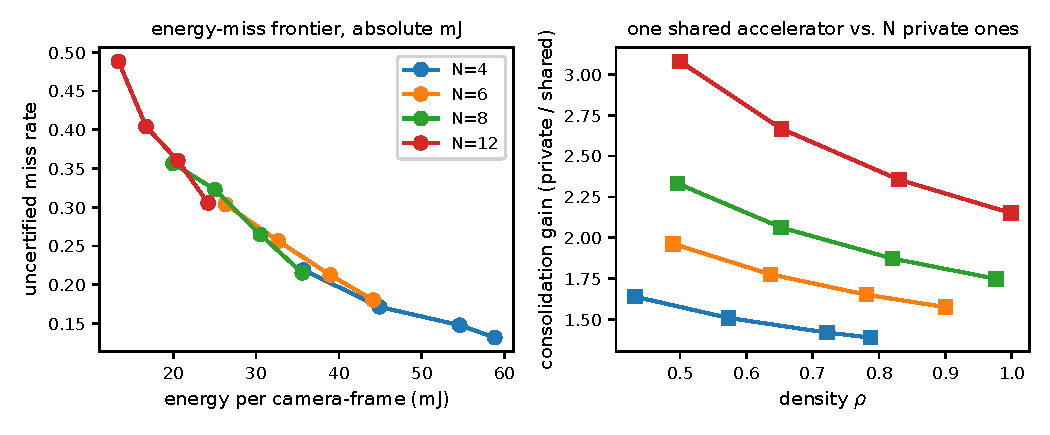
\includegraphics[width=\linewidth]{figures/fig_E7_energy.pdf}
\caption{Left: the energy--miss frontier in absolute mJ per camera-frame. Right: consolidation
gain --- the energy of $\Nc$ private accelerators divided by that of one shared accelerator.}
\label{fig:e7}
\end{figure}

Consolidation saves \numGainMin--\numGainMax$\times$ the energy, and the gain grows with fleet
size, because what consolidation removes is $(\Nc-1)E_{\mathrm{idle}}$ --- idle cost, not
inference cost. At twelve cameras and a half-density budget the fleet costs
\numTwelveHalfShared\,mJ per camera-frame on one shared box against \numTwelveHalfPrivate\,mJ with
one accelerator per camera, a factor of \numTwelveHalfGain. Because the scheduler pulls only the
frames it will inspect, the uplink and decode load scale with the busy fraction rather than with
the number of cameras; we do not model the network further.

\subsection{Sensitivity: no oracle, three corpora, and a latency cap}\label{sec:eval-sensitivity}
Three checks that a sceptical reader should demand (Figure~\ref{fig:e8}).

\begin{figure}[t]
\centering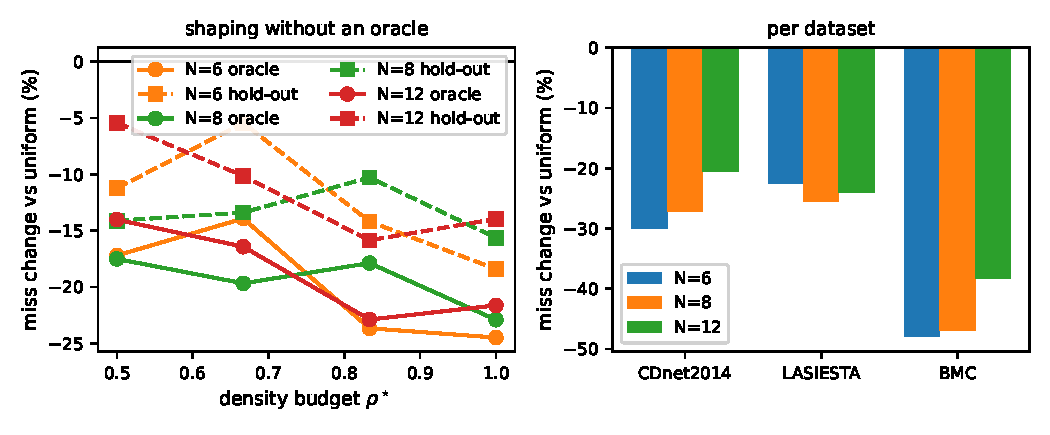
\includegraphics[width=\linewidth]{figures/fig_E8_sensitivity.pdf}
\caption{Left: budget shaping fitted on the evaluation half (oracle) versus fitted on the earlier
half and replayed on the later one (hold-out). Right: shaping gain by source dataset.}
\label{fig:e8}
\end{figure}

\emph{Shaping without an oracle.} In Section~\ref{sec:eval-frontier} the windows were fitted on
the same events used to evaluate them. We repeated the experiment with a temporal split: fit each
camera's windows on the first half of its history, replay on the second. Only
\numHoldoutVideos\ of the \numHoldoutTotal\ videos have at least one event in each half and can
support such a split, and we use those. Shaping still wins in \numHoldoutWins\ of
\numHoldoutCells\ configurations, reducing misses by \numHoldoutGain\,\% against
\numOracleGain\,\% for the oracle. Roughly \numOracleShare\,\% of the apparent benefit of shaping
is therefore an artefact of fitting on the evaluation data; the remainder is real. We report the
hold-out number as the honest one.

\emph{Foreground density.} A reader may object that this corpus is unusually busy. We split it by
source. Shaping wins in all \numPerDsWins\ of \numPerDsCells\ configurations, by
\numGainCdnet\,\% on CDnet2014, \numGainLasiesta\,\% on LASIESTA and \numGainBmc\,\% on BMC, with
zero certificate violations on each. Notably the gain is largest on BMC, which has the
\emph{longest} tail (90th percentile \numPninetyBmc\ frames). The effect therefore comes from the
dispersion of duration laws \emph{across} cameras --- exactly what Lemma~\ref{lem:worst} predicts
--- and not from foreground density.

\emph{Capping certified latency.} Capping the shaping grid at $K_{\max}=16$ instead of $64$ cuts
the worst certified latency from \numCapLatSixtyfour\ to \numCapLatSixteen\ slots and costs
\numCapCostPct\,\% relative in uncertified miss rate (\numCapMissSixteen\ against
\numCapMissSixtyfour\ at six cameras and $\dens^\star=5/6$). The latency--miss trade is a tunable
design parameter, not a fixed cost of the method.

\emph{A second baseline, and an explicitly unequal comparison.} Round robin is
\textbf{work-conserving}: its busy fraction is $1.0$ at every density budget, so it always spends
$100\,\%$ of the energy. On that footing it never violates a certificate when $\Nc\le K$ and it
achieves a lower miss rate than our scheduler at a half-density budget (\numRRMissSix\ against
\numRROursSix\ at six cameras, busy $1.0$ against busy $\dens^\star=0.5$). This is the one
comparison in the paper that is not made at equal energy, and it goes against us, so we state it
plainly rather than normalising it away. At $\dens^\star=1$ the two schedulers coincide. The contribution of this paper is therefore not that it beats
round robin on misses; it is that it lets an operator \emph{choose} a point on the energy--miss
frontier while keeping the certificate, and that it answers the sizing question when the windows
are heterogeneous, which round robin cannot.

% =====================================================================================
\section{Discussion and limitations}\label{sec:limitations}

\paragraph{The constructive gap is the main open problem.} Theorem~\ref{thm:capacity}(ii)
guarantees existence at $5/6$; the best scheduler we implement is the divisor wheel of
Section~\ref{sec:wheel}, which constructs a schedule for \numEoneWheelEightPct\,\% of the random
profiles in the band $(0.75,5/6]$ and is guaranteed only through the packing it finds, instance by
instance. We did \emph{not} implement the $7/10$ scheduler of \cite{chanchin1993schedulers} or the
$3/4$ scheduler of \cite{fishburn2002densities}. We attempted the former and stopped: the
construction is not stated in a form we could reproduce faithfully from the sources available to
us, and implementing a guessed version risks asserting a guarantee the code does not deliver.
Implementing either of them properly would narrow the gap measured in
Sections~\ref{sec:eval-schedulability} and \ref{sec:eval-dimensioning} without changing any
conclusion of this paper, and is the obvious next step. The divisor wheel is also restricted to
\emph{perfectly periodic} schedules; instances that are feasible but admit no perfectly periodic
schedule are out of its reach by construction, and no amount of wheel search will recover them.

\paragraph{Slot semantics.} A slot is a nominal per-frame service time, and all cameras are
assumed to produce frames at the slot rate. Variability in inference time is absorbed into two
upper-bound models --- switch cost (Section~\ref{sec:switch}) and blackouts
(Section~\ref{sec:blackout}) --- rather than measured directly. Frame-rate mismatch is handled by
flooring (Remark~\ref{rem:realperiods}).

\paragraph{No deployment.} This is a desk study. The scheduler is $O(\Nc K)$ to build and $O(1)$
per slot, so we expect no measurable runtime overhead, but we have not integrated it end to end,
and we make no claim about achieved throughput on a specific device. The energy figures come from
a model parameterised by two constants measured elsewhere.

\paragraph{Evaluation scope.} The corpus is replayed cyclically to fill the horizon, events cut by
the wrap are discarded, and a warm-up of $K_{\max}$ slots is excluded. The hold-out study uses
\numHoldoutVideos\ of \numHoldoutTotal\ videos. Churn is Bernoulli, swept over
\numEfiveLamLevels\ levels so that no conclusion rests on one parameter. The EDF-fit dimensioning
baseline is fitted on the evaluation trace and its zero violations must not be read as a
guarantee.

\paragraph{Exactness of the reference decisions.} The ``schedulable'' column of
Section~\ref{sec:eval-schedulability} comes from an exhaustive cycle search with a bounded state
budget, and \numEoneUndecided\ of the \numEoneInstances\ profiles exhaust that budget and are
excluded from the decided counts rather than being assumed one way or the other. The budget is a
state count and not a wall-clock limit, so the released code reproduces the same verdicts on any
machine.

\paragraph{Statistical caveats.} The admission-conservatism figure of \numConservPct\,\% reflects a
sampling design that over-weights densities above $5/6$ and is an upper bound, not an expected
operational refusal rate. The greedy allocator is within \numCsixGapMax\,\% of the grid optimum on
the instances we could enumerate exhaustively, which are smaller than deployed fleets.

\paragraph{What is not proved.} The model-group condition of Proposition~\ref{prop:groups} is a
sandwich, not a characterisation: sufficiency and necessity differ by $s$ slots. Our exhaustive
search found no feasible configuration in that gap, but we state this as an observation. The
factor-two dimensioning bound of Corollary~\ref{cor:dimensioning} is tight for our construction
and we do not know whether a constructive algorithm can approach $\lceil 1.2\dens\rceil$.

% =====================================================================================
\section{Conclusion}\label{sec:conclusion}

An edge box that must guarantee, and not merely optimise, per-camera coverage has a capacity that
can be written down: the sum of the reciprocals of the certificate windows must not exceed $5/6$,
and nothing better is available without solving an intractable instance. Around that one line we
built the pieces an operator needs --- an $O(1)$ admission test, a constructive scheduler that
holds the guarantee through camera churn, a water-filling rule for allocating the density budget
across cameras with different event statistics, a fleet-dimensioning procedure within a factor two
of optimal, and closed-form capacity reductions for model-switch cost and escalation blackouts.

On a public corpus of \numVideos\ videos and \numEvents\ events, the construction missed
\numEtwoCertMissed\ certified events out of \numEtwoCertTotal, budget shaping cut uncertified
misses by \numHoldoutGain\,\% out of sample at unchanged energy, and consolidating the fleet onto
one shared accelerator saved \numGainMin--\numGainMax$\times$ the energy of one accelerator per
camera. The results that did not go our way are equally informative: the $5/6$ threshold is a poor
bin-packing rule, an admission test without a matching construction still lets certificates break
under churn, and about \numOracleShare\,\% of the benefit of budget shaping vanishes once the
windows must be fitted on the past. Closing the gap between the density that is provably
schedulable and the density a deployable scheduler can actually realise is, in our view, the most
useful next step for this line of work.

% =====================================================================================
\appendix
\section{Proofs}\label{app:proofs}

\subsection*{Lemma~\ref{lem:worst}}
\begin{proof}
Consider a gap of camera $i$ between services at $a$ and $b=a+g$, $g\le\Ki$. Assign to this gap
the $g$ event onsets $s\in[a+1,b]$. The event $[s,s+\Dur-1]$ is missed exactly when it contains no
service. If $s+\Dur-1\ge b$ the service at $b$ lies in it; if $s+\Dur-1<b$ then no service lies in
it, since the previous service is at $a<s$ and every later service is at or after $b>s+\Dur-1$.
The missed onsets are therefore $s\in[a+1,b-\Dur]$, of which there are $\pos{g-\Dur}$. Averaging
over gaps with weights $g_j$ gives the stated equality. For the bound, $\pos{g-\Dur}=g\pos{1-\Dur/g}
\le g\pos{1-\Dur/\Ki}$ because $g\le\Ki$. Fix $\Dur<\Ki$; equality in every term requires
$\pos{1-\Dur/g_j}=\pos{1-\Dur/\Ki}$ for every $j$, hence $g_j=\Ki$ for all $j$. Conversely,
periodic service with gap $\Ki$ attains it. Taking the expectation over $\Dur\sim F_i$ gives
$\varepsilon_i(\Ki)$.
\end{proof}

\subsection*{Theorem~\ref{thm:capacity}(i) and (iii)}
\begin{proof}
(i) In any $T$ consecutive slots, a schedule with gaps at most $\Ki$ serves camera $i$ at least
$T/\Ki-1$ times. Summing over $i$ and bounding the total by $T$ gives $\dens\le1+\Nc/T$; let
$T\to\infty$.

(iii) We show the profile $A=(2,3,M)$ is infeasible for every $M$. Let $\mathcal{A}$ be the set of
slots serving camera 1. Its gaps are at most $2$, so the complement $\bar{\mathcal{A}}$ contains no
two consecutive slots. Cameras 2 and 3 can only be served in $\bar{\mathcal{A}}$. Suppose camera 3
is served at some slot $u$. Then $u\in\bar{\mathcal{A}}$, and since $\bar{\mathcal{A}}$ has no two
consecutive elements, $u-1\in\mathcal{A}$ and $u+1\in\mathcal{A}$. Now consider the window
$\{u-1,u,u+1\}$ of three consecutive slots: camera 2 has window $3$ and must be served in it, but
$u-1$ and $u+1$ serve camera 1 and $u$ serves camera 3 --- a contradiction. Hence camera 3 is
never served and $A$ is infeasible. Since $\dens(A)=5/6+1/M$, choosing $M>1/\varepsilon$ gives an
infeasible profile of density at most $5/6+\varepsilon$.
\end{proof}

\noindent
We verified (iii) independently by exhaustive state-graph search: all \numConeN\ profiles
$(2,3,M)$ for $M\le\numConeMmax$ are infeasible, the smallest density in the family being
\numConeRhoMin.

\subsection*{Theorem~\ref{thm:shaping}}
\begin{proof}
For fixed $\Dur$, $x\mapsto\pos{1-x\Dur}$ is the positive part of an affine function, hence convex;
expectation preserves convexity, so each $h_i$ is convex, and it is non-increasing, so the budget
binds at any optimum. The feasible set is a slice of a simplex, so Slater's condition holds and
the KKT conditions are necessary and sufficient. Since $h_i$ may be non-differentiable where $F_i$
has an atom at $1/x$, stationarity must be written with subgradients: $x^\star$ is optimal iff
there is $\lambda\ge0$ with $\lambda\in w_i\,\partial(-h_i)(x_i^\star)$ for all $i$ with
$x_i^\star<1$ and $\sum_i x_i^\star=\dens^\star$. Where $F_i$ has no atom at $1/x_i^\star$,
$h_i'(x)=-\mathbb{E}[\Dur\,\mathbf 1\{\Dur<1/x\}]$ and the condition reduces to the stated
water-filling equality. Finally, replacing $x_i^\star$ by $1/\lceil 1/x_i^\star\rceil\le x_i^\star$
only decreases the density, so the rounded profile still respects the budget.
\end{proof}

\subsection*{Proposition~\ref{prop:switch}}
\begin{proof}[Sufficiency]
Let $K_i'=\lfloor \Ki/(1+s)\rfloor$ and partition time into macro-slots of length $1+s$. If
$\sum_i 1/K_i'\le5/6$ then by Theorem~\ref{thm:capacity}(ii) there is a schedule $\sched'$ on
macro-slot indices meeting every $K_i'$-refresh property. Realise it by spending the first $s$
slots of macro-slot $m$ loading the model of camera $\sched'(m)$ and the last slot serving it. Two
consecutive services of camera $i$ occur at macro-slots $m_1<m_2\le m_1+K_i'$, hence at most
$(m_2-m_1)(1+s)\le K_i'(1+s)\le \Ki$ real slots apart.
\end{proof}

\begin{proof}[Exact homogeneous capacity]
Sufficiency: round robin has period $\Nc(1+s)\le K$. Necessity: fix a horizon $T$. Call a maximal
block of consecutive slots serving the same camera a \emph{run}; let camera $i$ have $R_i$ runs
and $n_i$ service slots, and write $n_i=R_i+e_i$ with $e_i\ge0$. Two consecutive runs of camera
$i$ start at most $(\text{run length}) - 1 + K$ apart, so $T\le n_i+R_i(K-1)$, that is
$R_iK+e_i\ge T$ and $R_i\ge(T-e_i)/K$. Every run other than the first is preceded by $s$ switch
slots, so
\[
T\;\ge\;\sum_i n_i+s\Big(\sum_i R_i-1\Big)\;=\;(1+s)\sum_i R_i+\sum_i e_i-s .
\]
Substituting $R_i\ge(T-e_i)/K$ gives
$T\ge \Nc(1+s)T/K+\sum_i e_i\big(1-(1+s)/K\big)-s$. Feasibility forces $K\ge 1+s$, so the
coefficient of $e_i$ is non-negative and the right-hand side is minimised at $e_i=0$, giving
$T\ge \Nc(1+s)T/K-s$. Dividing by $T$ and letting $T\to\infty$ yields $\Nc(1+s)\le K$. (A single
camera never switches, so $N_{\max}=1$ whenever $K\ge1$, independently of $s$.)
\end{proof}

\noindent
Note that the same argument with heterogeneous windows gives the necessary condition
$(1+s)\sum_i 1/\Ki\le1$ whenever $\min_i \Ki\ge 1+s$.

\subsection*{Proposition~\ref{prop:blackout}}
\begin{proof}
Fix a window $W=[t,t+\Ki-1]$. An escalation of length $\ell$ intersects $W$ exactly when its start
lies in $[t-\ell+1,\,t+\Ki-1]$, an interval of $\Ki+\ell-1$ slots. Starts are at least $P_e$ apart,
so at most $\lceil(\Ki+\ell-1)/P_e\rceil$ escalations intersect $W$, each blocking at most $\ell$
of its slots; trivially at most $\Ki$ slots of $W$ are blocked. Hence $W$ contains at least
$K_i''=\Ki-B_i$ available slots, and they are consecutive within the subsequence of available
slots. Run a schedule meeting every $K_i''$-refresh property on that subsequence, advancing the
pointer only on available slots; this requires no knowledge of future escalations. Since $W$
contains a run of $K_i''$ consecutive available slots, it contains a service of camera $i$.
\end{proof}

\noindent
We checked the budget against the true worst case over all escalation phases on
\numCfiveCells\ combinations of $(\ell,P_e,\Ki)$; it was never optimistic.

\subsection*{Corollary~\ref{cor:dimensioning}}
\begin{proof}
(1) On any bin, the rounded windows $\hat K_i$ are powers of two, hence pairwise divisible, so the
bin is a harmonic profile of density at most $1$ and is feasible by
Proposition~\ref{prop:structured}(a); the residue-wheel construction of Algorithm~\ref{alg:admit}
realises it. Since $\hat K_i\le K_i$, a $\hat K_i$-refresh schedule is also a $K_i$-refresh
schedule, so the original certificates hold.

(2) The item sizes $1/\hat K_i$ are dyadic, hence pairwise divisible. Process items in
non-increasing order. We claim first-fit-decreasing never leaves a bin partly filled while opening
a new one for an item that would fit. Indeed, when item $x$ is placed, every earlier item has size
a multiple of $x$, so the load of every open bin is a multiple of $x$; a bin with load $L<1$
therefore has residual capacity $1-L$ that is a multiple of $x$ and hence at least $x$, so $x$
fits in the first non-full bin. Consequently every bin except the last is filled exactly to $1$,
and $m=\lceil\sum_i x_i\rceil$.

(3) $\hat K_i>K_i/2$, so $1/\hat K_i<2/K_i$ and $\sum_i 1/\hat K_i<2\dens(A)$, whence
$m\le\lceil 2\dens(A)\rceil\le 2\lceil\dens(A)\rceil$.

(4) Each box must satisfy Theorem~\ref{thm:capacity}(i), so the densities of the parts are at most
$1$ each and their number is at least $\dens(A)$, hence at least $\lceil\dens(A)\rceil$.
\end{proof}

\noindent
We verified all four items on \numCfourTrials\ random profiles; the realised ratio
$m/\lceil\dens\rceil$ was \numCfourRatioMean\ on average and \numCfourRatioMax\ at worst.

% =====================================================================================
\section{Model groups}\label{app:groups}

\begin{proposition}[model groups]\label{prop:groups}
Partition the $\Nc$ cameras into $q\ge2$ \emph{model groups}; switching within a group is free and
between groups costs $s$. With a homogeneous window $K$:
\[
\underbrace{\Nc+q\,s\le K}_{\text{sufficient}}
\qquad\Longrightarrow\ \text{feasible}\ \Longrightarrow\qquad
\underbrace{\Nc+(q-1)\,s\le K}_{\text{necessary}} .
\]
\end{proposition}

The two conditions differ by exactly $s$ slots. We do not claim a characterisation, but we note
the evidence: over \numCthreeQtwo\ exhaustively decided configurations with $q\ge2$, both
conditions held without exception, and all \numCthreeBand\ configurations lying strictly between
them were infeasible.

\begin{proof}[Sufficiency]
Use the block-cyclic schedule of period $P=\Nc+qs$: in each period, visit the groups in a fixed
order, spending $s$ slots loading each group's model and then $|G_g|$ slots serving its cameras
one after another at no switch cost. Every camera is served once per period at the same offset, so
its gap is exactly $P\le K$.
\end{proof}
\begin{proof}[Necessity]
Let $W$ be any window of $K$ consecutive slots. By the refresh property every camera is served in
$W$, so $W$ contains at least $\Nc$ service slots and all $q$ groups appear in it. The sequence of
services restricted to $W$ therefore contains at least $q-1$ group changes, and each of them costs
$s$ slots lying between two services of $W$, hence inside $W$. Thus $K=|W|\ge \Nc+(q-1)s$.
\end{proof}

\noindent
For heterogeneous windows the same block schedule gives the following sufficient condition: assign
camera $i$ a multiplicity $m_i$ (a power of two), let group $g$ occupy a block of $L_g$ slots per
period and $P\ge\sum_g(s+L_g)$; if $m_iP+L_g-1\le K_i$ for every $i\in G_g$ then every certificate
holds.

% =====================================================================================

% =====================================================================================
\section*{CRediT authorship contribution statement}
\textbf{Dat Lam Quoc:} Conceptualization, Methodology, Formal analysis, Software, Investigation,
Data curation, Validation, Visualization, Writing -- original draft, Writing -- review \& editing.

\section*{Declaration of competing interest}
The author declares that he has no known competing financial interests or personal relationships
that could have appeared to influence the work reported in this paper.

\section*{Funding}
This research did not receive any specific grant from funding agencies in the public, commercial,
or not-for-profit sectors.

\section*{Declaration of generative AI and AI-assisted technologies in the manuscript
preparation process}
During the preparation of this work the author used Claude (Anthropic), via the Claude Code
command-line interface, in order to draft and copy-edit prose, to write and run the simulation and
proof-checking code, and to query the Crossref and arXiv interfaces used to verify the reference
list. After using this tool, the author reviewed and edited the content as needed and takes full
responsibility for the content of the published article.

\section*{Data availability}
The simulator, the proof-checking scripts, the result files from which every number in this paper
is generated, and the scripts that generate the tables, figures and bibliography are available at
\texttt{\numRepoUrl} (commit \numRepoCommit, tag \numRepoTag), released under an MIT licence. The
video corpora are third-party public datasets --- CDnet2014, LASIESTA and BMC --- and are cited
separately below. The per-event onset and duration annotations derive from the companion work
declared in Section~\ref{sec:intro}; the repository documents how to regenerate them and does not
redistribute the source video.

\bibliographystyle{elsarticle-num}
\bibliography{refs}

\end{document}
